\section{Vue globale}

\begin{figure}[H]
    \centering
    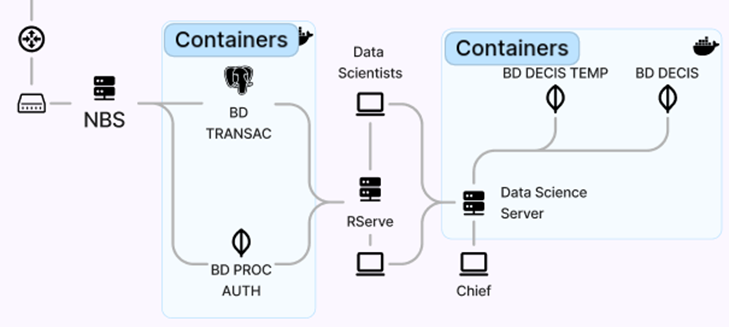
\includegraphics[width=\textwidth]{./img/thibault-VueGlobale.png}
    \caption{Vue globale du projet}
    \label{fig:thibault-global-view}
\end{figure}

\section{Data scientist application}

Cette application a été programmée en Java, développé avec le JDK17 et est gérée grâce à Gradle. Elle
utilise les frameworks suivants:

\begin{itemize}
    \item JavaFX afin de créer les interfaces graphiques. Utilisation du patron de conception Model-View-ViewModel.
    \item Spring boot afin de pratiquer l'injection de dépendance, et d'utiliser un fichier de properties pour configurer l'application sans avoir à la recompiler.
    \item Les librairies REngine et RServe afin de communiquer avec le serveur Rserve.
\end{itemize}

Afin de subvenir aux besoins du data scientist, cette application propose de travailler sur les bases de
données DB\_OPER\_PROC\_AUTH (MongoDB) et DB\_OPER\_TRANSACTIONS (PostGres) via RServe. C'est
le rôle du serveur RServe de récupérer les données dans les DBs et le les proposer au data scientist via
l'application.

De plus, cette application offre la possibilité de récupérer les résultats des opérations effectuées sur le
serveur Rserve, et de les manipuler au moyen de plusieurs interfaces JavaFX. Elle implémente les 3
méthodes d'exploration nde données suivantes :

\begin{itemize}
    \item Analyse de composantes principales
    \item Régression-corrélation multiple
    \item ACM
\end{itemize}

Une fois satisfait de l'étude des données, le data scientist peut tirer une conclusion l'envoyer au Data
Science Server via une socket utilisant TLS. Ce dernier les insère alors dans la base de données
DB\_DECIS\_TEMP.

\begin{figure}[H]
    \centering
    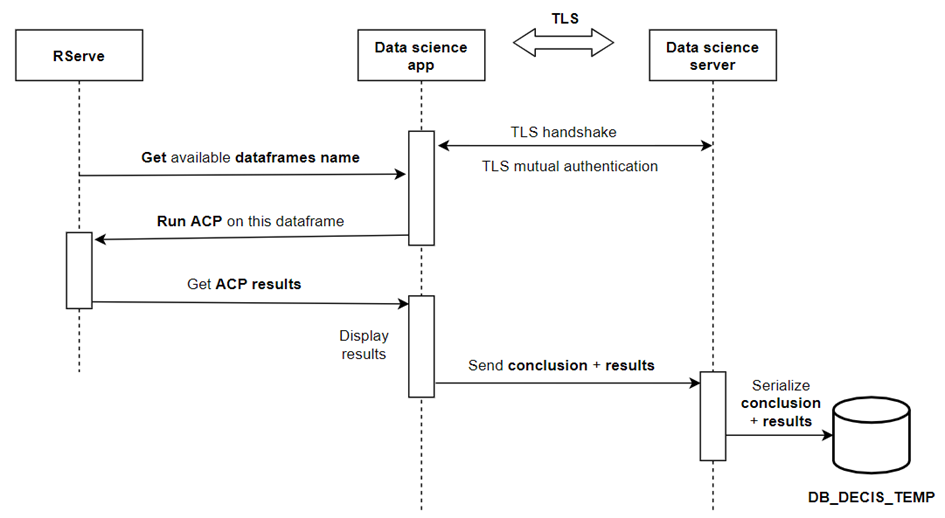
\includegraphics[width=\textwidth]{./img/thibault-DataScientistApp_1.png}
    \caption{Vue globale du projet}
    \label{fig:thibault-rserve-exchange}
\end{figure}

\section{Data Science Server}

C'est lui qui s'occupe de gérer les requêtes des data-scientist et du chief data-scientist. Pour ce faire, le
les requêtes sont gérées par un pool de thread, elles sont mises en attente dans une file en attendant
d'être exécutée par le pool.
Ce serveur est également chargé de sérialiser/désérialiser les conclusions dans les bases de données
DB\_DECIS\_TEMP et DB\_DECIS. Les accès concurrents sont pris en compte (un objet gérant les accès
aux DBs avec des méthodes 'synchronized').
Le type de requêtes autorisées vers ce serveur dépend du certificat du client (en fonction du Designated
Name plus précisément). Un chief data-scientist n'aura pas les mêmes droits qu'un data-scientist, et
n'importe qui ne peut se connecter au serveur et ce, grâce à l'authentification mutuelle de la couche
de sécurité TLS (le client doit lui aussi posséder un certificat, et le Data Science Server doit connaitre le
DN de ce certificat). Pour les plus curieux, s'en référer aux classes suivantes du projet 'data-minings-
apps' :

\begin{itemize}
    \item be.masi.g2.DataScientistServer.Tasks.TaskInstantiation
    \item be.masi.g2.DataScientistServer.ThreadPool.DataScientistServerThread
\end{itemize}

\section{Chief data scientist application}

Tout comme l'application des data scientist, ce logiciel utilise JavaFX, Spring boot ainsi que RServe et
REngine. L'application utilise également une socket utilisant TLS pour communiquer avec le Data
Science Server.
Elle passe par l'intermédiaire du Data Science Server afin de valider ou d'annuler les conclusions
stockées dans la base de données DB\_DECIS\_TEMP.

Récupération des conclusions :

\begin{figure}[H]
    \centering
    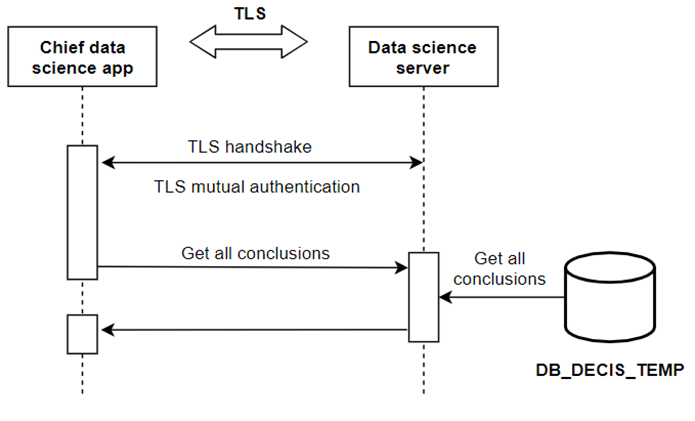
\includegraphics[width=\textwidth]{./img/thibault-DataScientistApp_2.png}
    \caption{Vue globale du projet}
    \label{fig:thibault-chief-app-retrieve}
\end{figure}

Validation d'une conclusion :

\begin{figure}[H]
    \centering
    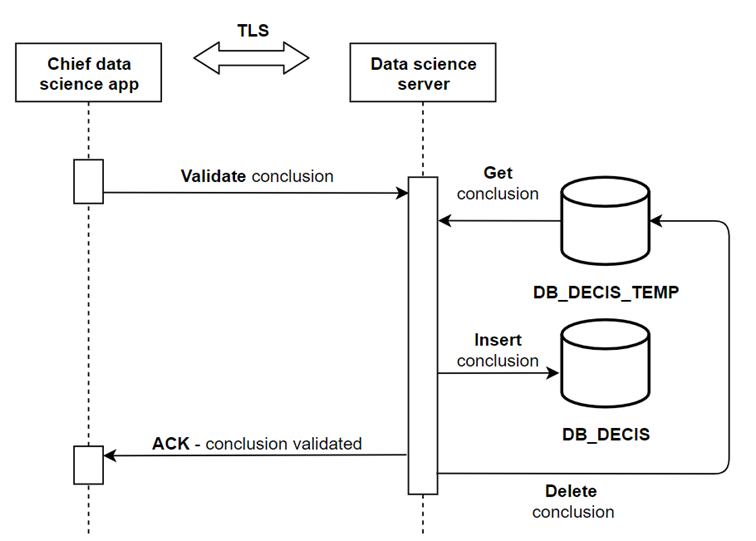
\includegraphics[width=\textwidth]{./img/thibault-DataScientistApp_3.png}
    \caption{Vue globale du projet}
    \label{fig:thibault-chief-app-validate}
\end{figure}

Annulation d'une conclusion :

\begin{figure}[H]
    \centering
    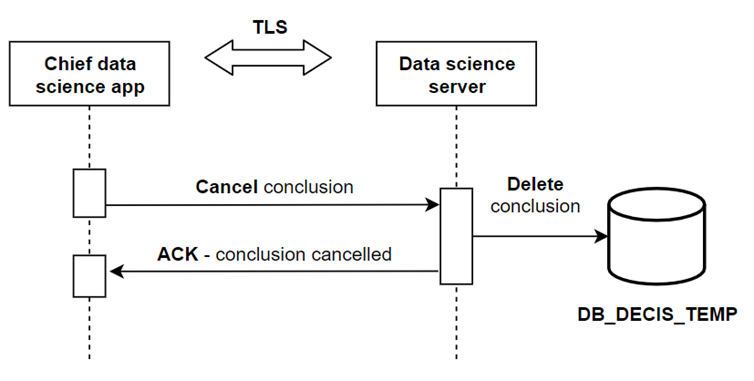
\includegraphics[width=\textwidth]{./img/thibault-DataScientistApp_4.png}
    \caption{Vue globale du projet}
    \label{fig:thibault-chief-app-cancel}
\end{figure}

\section{Serveur RServe}

Serveur prenant en compte les requêtes des data-scientist et du chef des data-scientist (via leurs apps respectives). Il est chargé de récupérer les données des bases de données \\ DB\_OPER\_PROC\_AUTH (MongoDB) et DB\_OPER\_TRANSACTIONS (PostGres) et de les convertir en dataframes exploitables par les data-scientist. De fait, les données contenues dans les bases de données ne sont pas utilisables par le framework 'FactoMineR' (package R consacré à l'exploration de donnée).

Ce script porte le nom de 'ConvertAuthenticationToDataFrame.R' et est disponible dans l'archive jointe.

\subsection{Exemple de traitement des données}

On commence tout d'abord par récupérer les données dans l'une des bases de données. En l'occurrence, la DB\_OPER\_PROC\_AUTH (MongoDB) :

\begin{listing}[H]
    \begin{minted}{r}
library(mongolite)

connection_string = 'mongodb://127.0.0.1:27017'
clientsCollection = mongo(collection="clients", db="DB_OPER_PROC_AUTH", url=connection_string)
clients <- clientsCollection$find()

clientDf <- as.data.frame(clients)
    \end{minted}
    \caption{Récupération des données depuis la DB MongoDB}
    \label{listing:thibault-retrieve-data}
\end{listing}

En l'état des choses, la dataframe clientDf possède la même structure que la collection 'clients' de la
base de données. On a ici récupéré la liste des clients. Chaque document est structuré comme suit :

\begin{listing}[H]
    \begin{minted}{r}
- Clients :
    - Date naissance
    - Sexe
    - Banques
        - Nom
    - OTPs:
        - Date-heure demande
        - âge du client au moment de la demande (automatique)
        - compteur essai
        - temps authentification (date-heure reception - date-heure demande)
        - décision
        - nouvel essai nécessaire ?
        - nombre d'essais dépassé ?
    - SMSs :
        - Data-heure demande
        - âge du client au moment de la demande (automatique)
        - envoi par réseau ou par SMS ?
        - temps authentification (date-heure réception - date-heure demande)
        - hors délai ?
        - décision
    - E-mails :
        - date-heure demande
        - âge du client au moment de la demande (automatique)
        - montant transaction envisagée
        - HTTP ou HTTPs
        - temps authentification (date-heure reception - date-heure demande)
        - hors délai ?
        - décision
    - EIDs :
        - date-heure demande
        - âge du client au moment de la demande (automatique)
        - temps authentification (date-heure reception - date-heure demande)
        - décision
    \end{minted}
    \caption{Structure des données du document}
    \label{listing:thibault-structure-db}
\end{listing}

La structure de cette base de données reste à améliorer. De fait, un document client stocke toute ses
authentifications. Nous sommes conscients qu'il y a un petit problème d'optimisation de place
(certaines données sont dupliquées) et que cela risque également de coincer sur le long terme au
niveau de la taille maximale d'un document sur MongoDB (16Mo maximum par document). Il aurait
fallu créer une collection par type d'authentification. Malheureusement, ayant trop peu d'expérience
en NoSQL, et s'étant rendu compte de l'erreur trop tard (toute l'infrastructure a déjà été construite
autour de cette BD), nous n'avons pas eu le temps de rectifier cela.

Mais revenons-en au traitement de la dataframeclientDf. Pour notre exemple, nous allons créer une
dataframe exploitable par R qui possède les colonnes suivantes : NbreBanque - Genre Age - NbrEID -
NbrEmail - NbrOTP – NbrSMS.

\begin{listing}[H]
    \begin{minted}{r}
nbrAuthDf = data.frame()

clientNbr = nrow(clientDf)

for(i in 1:clientNbr){
    client = clientDf[i,]
    bankNbr = nrow(client$banks[[1]])
    gender = client$gender
    age = as.integer(as.numeric((Sys.time() - client$birthday))/365.25)
    eidAuthNbr = nrow(client$eidAuthentication[[1]])
    otpAuthNbr = nrow(client$otpAuthentication[[1]])
    smsAuthNbr = nrow(client$smsAuthentication[[1]])
    mailAuthNbr = nrow(client$mailAuthentications[[1]])
    nbrAuthDf <- rbind(nbrAuthDf, list(bankNbr, gender, age, eidAuthNbr, mailAuthNbr, otpAuthNbr, smsAuthNbr))
}
colnames(nbrAuthDf) <- c("BankNbr", "Gender", "Age", "EIDAuthNbr", "MailAuthNbr", "OTPAuthNbr", "SMSAuthNbr")
    \end{minted}
    \caption{Récupération des données depuis la DB MongoDB}
    \label{listing:thibault-r-code}
\end{listing}

\subsubsection{Remarque}

C'est le chef des data-scientist qui a pour rôle de lancer le script de récupération et de traitement de ces données :

\begin{figure}[H]
    \centering
    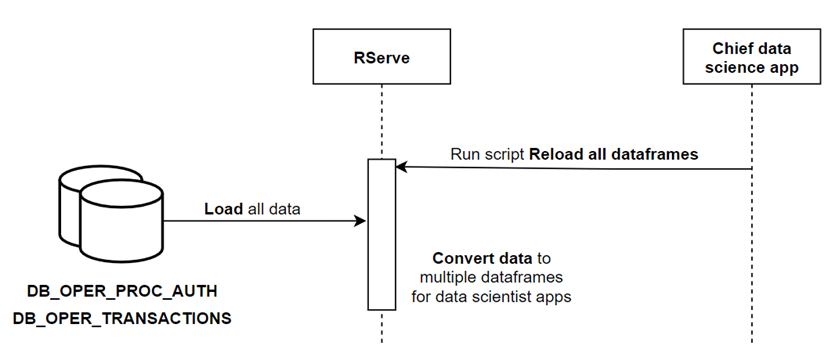
\includegraphics[width=\textwidth]{./img/thibault-Serveur_RServe.png}
    \caption{Échange des données avec l'application Chief}
    \label{fig:thibault-server-rserve}
\end{figure}

\section{Tests}

\subsection{Test de l'API}

Le bon fonctionnement de l'API permettant d'insérer les transactions (NBS) a été testé à l'aide du
framework Cucumber. Cet outil permet de générer des scénarios de texte dans un langage
compréhensible par tout le monde et de relier cette documentation à des fonction java permettant de
tester ces même scénarios (et ainsi, assurer la véracité du scénario). On se retrouve alors avec une
documentation vivante du projet.

En l'occurrence, voici les scénarios qui ont été testés\footnote{Le langage utilisé ci-dessus est appelé Gherkin, et est composé de 'Given' - 'When' - 'Then'. Chacune
de ces lignes est reliée à une fonction qui sera exécuté lors du test du scénario.} :

\begin{figure}[H]
    \centering
    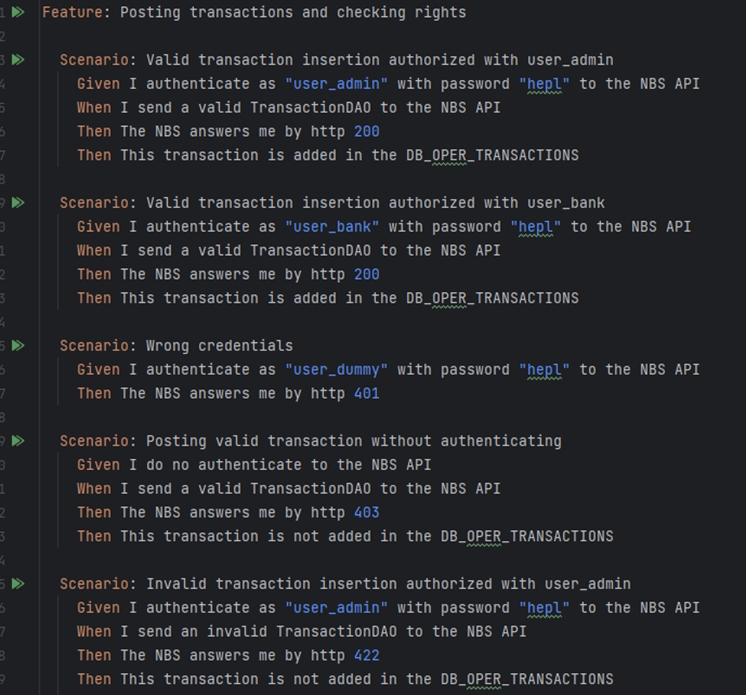
\includegraphics[width=\textwidth]{./img/thibault-Tests_1.png}
    \caption{Représentation des tests unitaires}
    \label{fig:thibault-unit-testing-01}
\end{figure}

Le lien est effectué dans le code à l'aide d'une annotation placée juste avant la définition de la
fonction :

\begin{figure}[H]
    \centering
    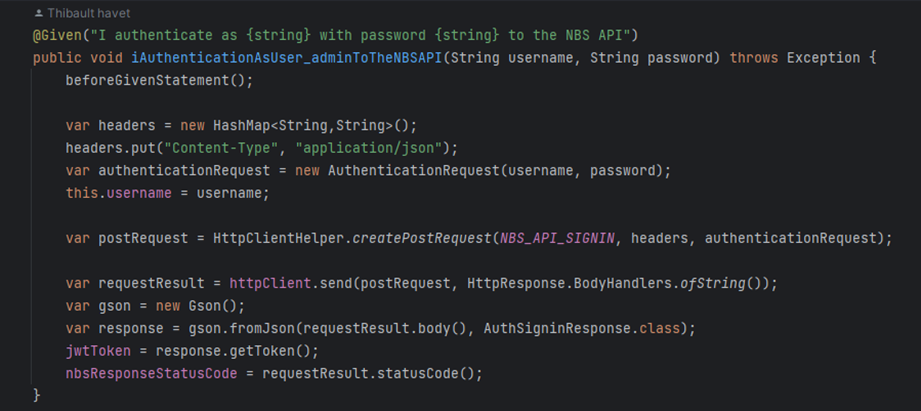
\includegraphics[width=\textwidth]{./img/thibault-Tests_2.png}
    \caption{Code d'un test unitaire en Java}
    \label{fig:thibault-unit-testing-02}
\end{figure}

\subsection{Génération de données bruitées}

Le test de la partie DB\_OPER\_XXX <-> RServe <-> data-scientist-app repose sur un code de génération de données contenu dans le National Bank Server. Cette application a pour but de remplir les 2 bases de données 'DB\_OPER\_XXX' avec des données factices.

Cependant, ces données ne peuvent pas simplement être générée aléatoirement, et il a fallu implémenter plusieurs outils permettant de générer un bruit gaussien (voir le package be.masi\_liege\_g2\_2223.data\_generation.randomizer du projet national-bank-server).

La major partie de ces outils reposent sur un générateur de nombre aléatoire avec une fonction de répartition gaussienne. Par exemple, si l'on souhaite générer un nombre dans un certain intervalle défini par une borne min et une borne max, le calcul est le suivant :

\begin{listing}[H]
    \begin{minted}{java}
// …
do{
    result = Math.round(mean + calculateNoise());
} while(result < min || result > max);
// …

private double calculateNoise(){
    return stdDev * random.nextGaussian();
}
    \end{minted}
    \caption{Génération d'une borne min-max dans un interval}
    \label{listing:thibault-gen-noise}
\end{listing}

Avec 'random' un java.util.Random qui a été initialisé avec 'new Date().getTime()' et la fonction nextGaussian qui renvoie un flottant à double précision aléatoire généré par une Gaussien de moyenne 0 et de variance 1. Afin de pouvoir modifier l'écart type et la moyenne de cette fonction random.nextGaussian(), on multiplie le résultat par l'écart-type voulu (stdDev) et lui ajoute la moyenne voulue (mean).

Une fois ces outils mis en place, il fut aisé de générer les données (voir la classe be.mas\_liege\_g2\_2223.applications.DataGeneration ainsi \\ que le package be.masi\_liege\_g2\_2223.data\_generation du projet national-bank-server).

\subsubsection{Exemple}

On génère des données comme suit du côté du National Bank Server :

\begin{listing}[H]
    \begin{minted}{r}
// -----------------------------
// HOMME de 45 à 75 ans
// -----------------------------
// +EID
// +EMail
// temps auth =~ 25 000ms
// 2 banques
// -----------------------------
// FEMME de 45 à 75 ans
// -----------------------------
// +EID
// +OTP
// temps auth =~ 20 000ms
// 2 banques
// -----------------------------
// HOMME de 20 à 40 ans
// -----------------------------
// +EMail
// +SMS
// temps auth =~ 10 000ms
// 1 banque
// -----------------------------
// FEMME de 20 à 40 ans
// -----------------------------
// +EMail
// +SMS
// temps auth =~ 10 000ms
// 1 banque
    \end{minted}
    \caption{Génération d'une borne min-max dans un interval}
    \label{listing:thibault-generated-data-scheme}
\end{listing}

Ci-dessus, '+Email' signifie que la personne s'authentifie beaucoup plus souvent par Email. En
l'occurrence, '+Email' signifie que sur 260 authentifications, la personne s'authentifiera en moyenne
100 fois par Email (fonction de répartition Gaussienne avec une moyenne de 100 et un écart-type de
20).

On génère :

\begin{itemize}
    \item 150 femmes de 20 à 40 ans
    \item 150 hommes de 20 à 40 ans
    \item 100 femmes de 45 à 75 ans
    \item 100 hommes de 45 à 75 ans
\end{itemize}

Une fois injectée dans des 2 bases de données et passées au serveur RServe, on peut vérifier que les données reflètent ce qui a été établit plus haut. Ici, le serveur RServe a créé un dataframe nommée 'nbrAuthDf' qui permet d'étudier les préférences d'authentification d'une personne. Elle est composée des colonnes suivantes :

NbreBanque - Genre - Age - NbrEID - NbrEmail - NbrOTP - NbrSMS

Après avoir récupéré les données sur l'application du data-scientist (via le serveur RServe) on commence par faire une ACP afin d'établir des corrélations entre des variables quantitatives (elles le sont toute, excepté le genre).

\begin{figure}[H]
    \centering
    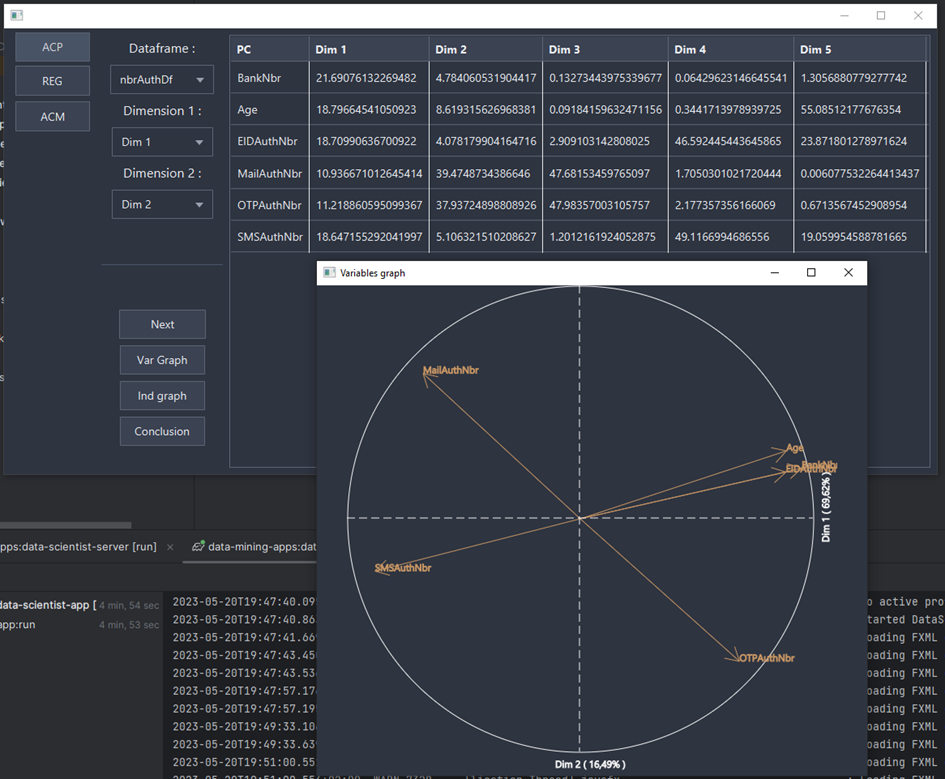
\includegraphics[width=\textwidth]{./img/thibault-Tests_Exemple_1.png}
    \caption{ACP de variables quantitaives}
    \label{fig:thibault-ex-01}
\end{figure}

On constate que la dimension 1 prend énormément d'inertie (69,62\% de l'inertie totale), elle est donc
significative, et permet de mettre en exergue beaucoup d'informations.

De plus, toutes les variables sont bien projetées (loin du centre du cercle).

On observe que l'age, le nombre d'authentification EID et le nombre de banque sont fortement
corrélées. De plus, le nombre d'authentification par SMS et le nombre d'authentification par EID sont
corrélées négativement. Il en va de même avec l'authentification par Mail et avec OTP. De fait, dans les
données générées plus haut, quel que soit la catégorie (jeune/âgé homme/femme), personne ne
s'authentifie souvent par mail ET par OTP (il en va de même pour SMS et EID).

De ce graphique, on en tire également la conclusion que les variables 'Age', 'EIDAuthNbr', 'BankNbr' et
'SMSAuthNbr' (négativement) contribuent fortement à la dimension 1. Par conséquent, les personnes ayant un X positif sur le graphique des individus auront tendance à être plus âgé, à avoir 2 banques, et
à s'authentifier par EID, ou par OTP qui contribue lui aussi, mais un peu moins, à la dimension.

Cependant, s'ils ont un X négatif, ils auront plutôt tendance à être jeunes et à utiliser l'authentification
par mail et SMS.

On retrouve donc bien les caractéristiques établies dans les données factices.

Petite parenthèse sur la variable 'Email' : celle-ci se situe plus à gauche, alors que certaines personnes
âgées l'utilisent également. De fait, il y a 300 jeunes qui ont été généré, pour seulement 200 personnes
plus âgées, et seules 100 personnes l'utilisent.

Passons maintenant à la régression-corrélation multiple. On commence par une régression à une variables explicative. On va tenter d'expliquer la variable 'SMSAuthNbr' par l'age :

\begin{figure}[H]
    \centering
    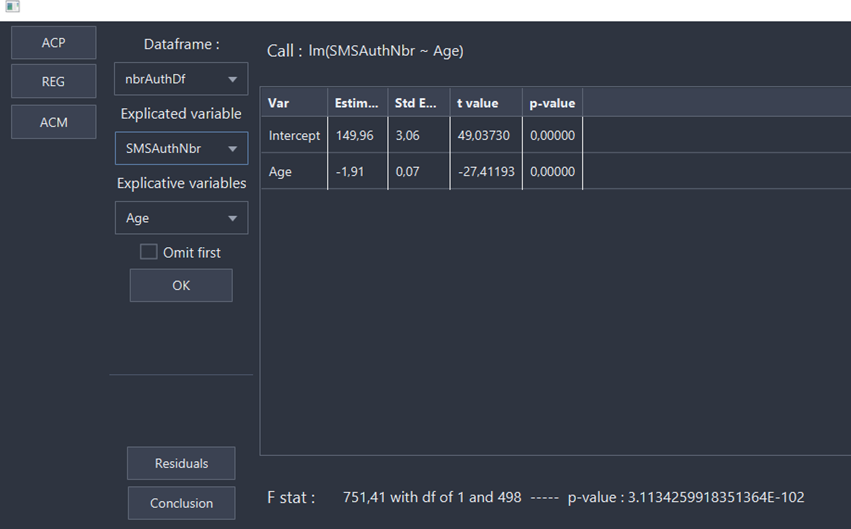
\includegraphics[width=\textwidth]{./img/thibault-Tests_Exemple_2.png}
    \caption{p-values de Fischer}
    \label{fig:thibault-ex-02}
\end{figure}

On constate que le modèle est fiable (p-value de Fisher avec vraiment infime) et le paramètre 'Age'
du modèle est également très fiable (p-value de 0).

Un petit peu plus compliqué maintenant, on va tenter d'expliquer la variable 'SMSAuthNbr' en
fonction des 3 variables qui lui sont corrélées négativement :

\begin{figure}[H]
    \centering
    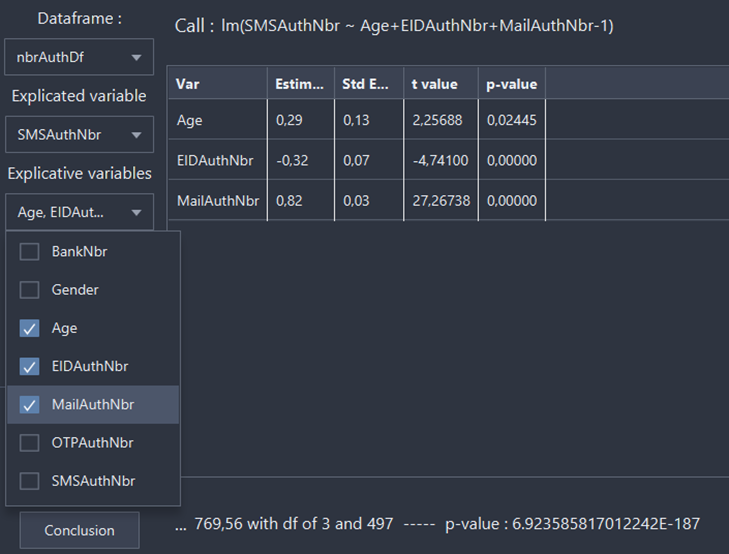
\includegraphics[width=\textwidth]{./img/thibault-Tests_Exemple_3.png}
    \caption{p-values de Fischer}
    \label{fig:thibault-ex-03}
\end{figure}

On obtient une p-value de Fisher encore plus petite. Les coefficient 'Age', 'EIDAuthNbr'et
'MailAuthNbr'sont également très fiable (p-value valant 0 ou en étant proche).

Il n'est ici pas possible de réaliser une ACM en raison du nombre de variables qualitative. Pour ce
faire, il faut s'en référer à un autre jeu de données :

\begin{listing}[H]
    \begin{minted}{r}
// -----------------------------
    // HOMME AGE
    // -----------------------------
    // +EID
    // +EMail
    // +Capricioso
    // +Du chef
    // 60% de personnes divorcées - 30% marriées
    // + delMolin et +Andrea
    // -----------------------------
    // FEMME AGEE
    // -----------------------------
    // +OTP
    // +Mezzo mezzo
    // +Du chef
    // 60% de personnes divorcées - 30% marriées
    // + pinocchio et +Andrea
    // -----------------------------
    // YOUNG PEOPLE
    // -----------------------------
    // +SMS
    // +Margerita
    // +Calzone
    // 40% de single - 30% married - 20% divorced
    // +pizza hut
    \end{minted}
    \caption{Génération d'une borne min-max dans un interval}
    \label{listing:thibault-another-data-set}
\end{listing}

Même procédé que le précédent (100 personnes plus âgées de chaque sexe, et 300 jeunes). Le
serveur RServe transforme ces données en la dataframe suivantes :

"Amount", "Account Previous State", "Merchant", "Gender", "Age", "Marital Status", "Monthly
Salary", "Auth type", "Product" (la variables product est ici composées de pizza).

On supprime donc toutes les colonnes quantitatives, on se retrouve alors avec les colonnes
suivantes : "Merchant", "Gender", "Marital Status", "Auth type", "Product"

On effectue ensuite l'ACM et on en étudie les valeurs propres :

\begin{figure}[H]
    \centering
    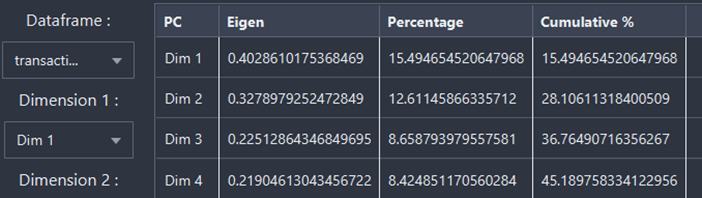
\includegraphics[width=\textwidth]{./img/thibault-Tests_Exemple_4.png}
    \caption{Résultat de l'ACM}
    \label{fig:thibault-ex-04}
\end{figure}

Les 2 premières dimensions sont plutôt convaincantes, prenant 28\% de l'inertie totale, ce qui n'est
pas rien pour une ACM (puisque l'inertie est diluée dans les modalités rajoutées).

\begin{figure}[H]
    \centering
    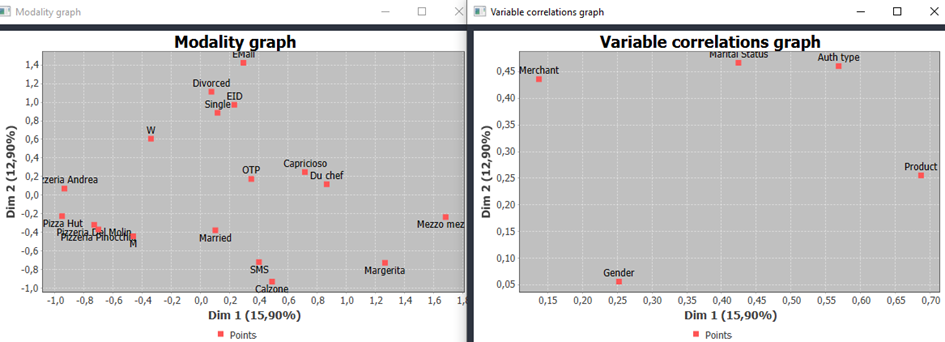
\includegraphics[width=\textwidth]{./img/thibault-Tests_Exemple_5.png}
    \caption{Les carrés des corrélations et le graphique des modalités (pour la dim. 1 et 2)}
    \label{fig:thibault-ex-05}
\end{figure}

On observe par exemple que les personnes qui s'authentifient par SMS mangent des calzone (lesau
jeunes), que les personnes qui mangent des pizzas 'Du chef' consomment également des pizzas
'Capricioso' (les homes plus âgés).

Cependant, on remarque quelques incohérences comme les personnes qui utilisent EID qui ont
tendances à être divorcées ou célibataire. Pareil pour les marchants qui sont tous collés les uns aux
autres.

\subsection{A refaire}

La réalisation de cette partie du projet intégrée fut beaucoup trop longue, le développement de la
branche data-scientist (NBS + DSS ainsi que les 2 applications et la gestion des 4 bases de données) a
pris plus de 60h de développement. Si cela était à refaire :

\begin{itemize}
    \item Nous n'aurions pas utilisé Rserve. De fait, cette librairie souffre de 2 défauts majeurs :
    \begin{itemize}
        \item Le débogage est inexistant. De plus, quel que soit l'erreur commise lors de l'exécution d'une commande depuis java, le serveur envoie le code d'erreur 127 sans aucun autre message.
        \item La récupération des données depuis R vers java (et inversement) est un travail d'orfèvre. En effet, il faut appeler une méthode par champs à récupérer, ce qui peut mener à des fonctions gargantuesque au code immonde (voir la classe be.masi.g2.
        REngineRServeUtils.Utils.RDataMediator).
    \end{itemize}
    \item Nous aurions utilisé les interfaces de REngine pour afficher les résultats. En l'état des choses,
    tous les résultats des méthodes d'exploration de données (ACP, régression linéaire multiple,
    ACM) sont extraits de R, convertit en un objet java et ensuite affiché dans une fenêtre JavaFX
    (en utilisant la librairie JFreeChart ou non).
    Cependant, la conception de chacune de ces fenêtres nous a pris beaucoup trop de temps.

    \textbf{NB} : En réalité, il aurait été plus judicieux d'utiliser des notebooks. De fait, ceux-ci présentent
une plus grande flexibilité (le data-scientist peut écrire lui-même le code et utiliser les
méthodes qu'il désire, sans devoir passer par une nouvelle fenêtre JavaFX pour chaque
afficage). Une fois la conclusion tirée, le Data-Science-Server aurait stocké le notebook dans la
DB\_DECIS\_TEMP, etc, etc.

    \item Nous aurions optimisé le menu de l'application data-scientist. De fait, la fenêtre de démarrage
    charge toutes les informations de chacune des conclusions, ce qui n'est pas optimisé. Il aurait
    fallu charger les informations strictement nécessaires telles que le titre de la conclusion,
    l'auteur, la date de la conclusion, …
\end{itemize}
